\documentclass[12pt,a4paper]{article}

% Packages
\usepackage[utf8]{inputenc}
\usepackage[english]{babel}
\usepackage{amsmath,amssymb,amsthm}
\usepackage{graphicx}
\usepackage[margin=1in]{geometry}
\usepackage{natbib}
\usepackage{hyperref}
\usepackage{booktabs}
\usepackage{multirow}
\usepackage{array}
\usepackage{algorithm}
\usepackage{algpseudocode}

% Formatting
\setlength{\parindent}{0pt}
\setlength{\parskip}{10pt}
\hypersetup{
    colorlinks=true,
    linkcolor=blue,
    citecolor=blue,
    urlcolor=blue
}

% Title and Authors
\title{\textbf{SynthIE: A Hierarchical Multi-Agent Framework for the Automated Synthesis of Industrial Engineering Research}}

\author{
    Brigitte Castañeda \\
    \textit{Industrial Engineering Department} \\
    \textit{[University Name]} \\
    \texttt{brigitte.castaneda@[university].edu}
    \and
    Jaime Polanco-Jiménez \\
    \textit{Industrial Engineering Department} \\
    \textit{[University Name]} \\
    \texttt{jaime.polanco@[university].edu}
}

\date{\today}

\begin{document}

\maketitle

\begin{abstract}
This research addresses the critical gap between general-purpose Large Language Models (LLMs) and the specialized, multi-dimensional requirements of Industrial Engineering (IE) research. We propose \textbf{SynthIE}, a hierarchical Multi-Agent System (MAS) built on the Google Agent Development Kit (ADK). SynthIE utilizes a modular architecture comprising four specialized Knowledge Clusters: Mathematical/Economic, Physical/Production, Operational/Systemic, and Human/Social. By leveraging ADK primitives—Sequential, Parallel, and Loop agents—the framework enforces methodological triangulation, ensuring that every research output is validated against quantitative optimization, financial viability, and safety/ergonomic constraints. We demonstrate the framework's efficacy through three validation experiments: qualitative policy synthesis for climate risk, financial triangulation for cost-of-capital estimation, and iterative machine learning optimization for building energy consumption. SynthIE shifts the paradigm from simple text generation to agent-aided knowledge discovery, providing a robust pathway for automating the production of high-impact, ``Gold Standard'' IE research that balances scientific explanation with engineering praxis.

\textbf{Keywords:} Multi-Agent Systems, Industrial Engineering, Large Language Models, Knowledge Engineering, Methodological Triangulation, Agent Development Kit
\end{abstract}

\section{Introduction: The Epistemological Gap in IE Research}

The ``Gold Standard'' of Industrial Engineering (IE) research requires a delicate balance between two distinct epistemologies: \textit{scientific explanation} (knowledge-that) and \textit{engineering praxis} (knowledge-how). Industrial Engineering is formally defined as the design, improvement, and installation of integrated systems of people, materials, information, equipment, and energy, drawing upon specialized knowledge in the mathematical, physical, and social sciences to specify, predict, and evaluate results.

\subsection{The Hook: Bridging Two Worlds}

On one side is the scientific demand for systematic explanation and universal laws; on the other is the engineering mandate for praxis—the transformation of a situation through the design of artifacts. A solution for Supply Chain Management is fundamentally flawed if it ignores Information Engineering data structures or violates OSHA safety regulations. This dual nature creates a unique challenge for automation.

\subsection{The Gap: Current AI Limitations}

While current Large Language Models (LLMs) possess general linguistic capabilities, they lack the specific ontological grounding required to navigate the diverse ``Knowledge Areas'' of the profession—ranging from the mathematical rigor of Operations Research to the biomechanical constraints of Ergonomics. The fundamental limitation of current LLMs in IE research manifests in four critical failure modes that directly impact research productivity and publication quality.

First, when addressing Supply Chain optimization problems, monolithic models default to qualitative reasoning, systematically ignoring the mathematical necessity of inventory control methodologies such as Economic Order Quantity (EOQ) and Make-to-Stock versus Make-to-Order decision frameworks. This omission renders the output unsuitable for publication in quantitative IE journals such as \textit{Production and Operations Management} or \textit{Manufacturing \& Service Operations Management}, where mathematical rigor is a non-negotiable requirement. A researcher attempting to use such output must then spend an additional 20-40 hours manually formulating the optimization models, negating any time savings from AI assistance.

Second, and perhaps more problematically, these models apply deterministic logic to inherently stochastic social systems, failing to recognize that organizational behavior does not obey universal laws but emerges from the complex interplay of human agency, cultural norms, and power dynamics. When tasked with designing a change management intervention, a standard LLM will propose mechanistic solutions (``implement new workflow, train employees, measure KPIs'') that ignore the insights of Social Systems Engineering—namely, that social organizations are ``artificial systems'' requiring heuristic steering rather than optimization. This epistemological mismatch results in research that is rejected during peer review for failing to account for human complexity.

Third, current models fail to account for multimodal rigor. A typical IE research paper requires the synthesis of disparate methodologies: a single study might need to optimize an XGBoost hyperparameter (Machine Learning), reverse-engineer a Weighted Average Cost of Capital from auction bid data (Engineering Economics), and draft a nuanced climate adaptation policy (Qualitative Management). A monolithic LLM cannot maintain methodological coherence across these domains without suffering from context drift and hallucination, particularly when the context window exceeds 50,000 tokens. The result is internally contradictory research where, for example, the financial analysis assumes a 10\% discount rate while the optimization model uses 5\%, or where the machine learning feature selection contradicts the domain knowledge encoded in the qualitative sections.

Fourth, existing tools lack the governance mechanisms required to handle the confidential deal data inherent to IE finance and proprietary manufacturing processes. Industrial Engineering research frequently involves sensitive information: capital investment decisions, supplier contract terms, production cost structures, and workforce compensation data. Current AI systems operate as ``black boxes'' that ingest all provided data without human oversight, creating unacceptable intellectual property risks for corporate-sponsored research. This privacy concern has led many organizations to ban the use of AI tools entirely, preventing researchers from benefiting from automation.

\subsection{The Contribution: SynthIE}

We propose \textbf{SynthIE}, an expert system that codifies the specific characteristics of the IE discipline into a retrieval-augmented, multi-agent architecture. Unlike generic writing assistants, SynthIE addresses each of the four failure modes through targeted architectural innovations.

To solve the mathematical rigor problem, SynthIE formulates a \textbf{Hierarchical Task Decomposition} model where an Orchestrator agent analyzes the research directive and routes quantitative problems to a specialized Quantitative Engine. This engine contains dedicated agents for Operations Research (formulating LP models, queuing systems, and simulations), Engineering Economics (conducting NPV/IRR analysis with explicit cash flow modeling), and Information Engineering (ensuring data integrity through proper database design and analytics pipelines). By compartmentalizing these domains, the system prevents the ``qualitative drift'' that plagues monolithic models.

To address the epistemological mismatch in social systems, SynthIE implements a separate Social Systems Engine that operates on fundamentally different logic. Rather than seeking optimal solutions, this engine uses ADK's \texttt{LoopAgent} primitive to iteratively generate and refine heuristic strategies. When evaluating a proposed factory layout, for example, the Quantitative Engine might optimize material flow to minimize handling costs, but the Social Systems Engine will then critique this solution by asking: ``Will the organizational culture accept this disruption? Does the layout account for informal communication patterns? Have we considered the union's perspective on workstation redesign?'' This dual-engine approach ensures that hard systems and soft systems are treated with appropriate methodologies.

To achieve multimodal rigor, SynthIE utilizes ADK's \texttt{ParallelAgent} primitive to perform ``Methodological Triangulation.'' When estimating a financial parameter such as the Weighted Average Cost of Capital, three sub-agents execute simultaneously: a MarketAgent applies Capital Asset Pricing Model logic to market data, a SurveyAgent analyzes expert interview transcripts, and an AuctionAgent reverse-engineers discount rates from historical bid data. A downstream SynthesizerAgent then aggregates these estimates into a robust range with explicit uncertainty quantification, satisfying the validation requirements of top-tier journals. This parallel architecture prevents the context drift that occurs when a single agent attempts to sequentially process multiple methodologies.

Finally, to solve the privacy problem, SynthIE implements a \textbf{Human-in-the-Loop Policy Engine} that intercepts any tool call attempting to access confidential data. When the system requires proprietary information (e.g., actual supplier contract terms, real production costs), it pauses execution and prompts the researcher to manually sanitize the data before ingestion. This governance mechanism allows organizations to benefit from AI-assisted research without compromising intellectual property, transforming SynthIE from a ``black box'' into a ``glass box'' system where every data access is auditable.

Collectively, these innovations shift the paradigm from computer-aided writing to \textit{agent-aided knowledge discovery}. Rather than generating generic text that researchers must then manually validate, SynthIE ensures methodological rigor \textit{during} generation by encoding the acceptance criteria of top-tier IE journals directly into the agent workflows. The system validates every research output against the specific characteristics of the relevant knowledge areas, from the atomic structure of materials in Manufacturing Engineering to the strategic leadership frameworks in Engineering Management, ensuring that the final product meets the ``Gold Standard'' for publication.

\section{Literature Review and Positioning}

Current automated research tools fall into two categories: ``Monolithic LLMs'' (e.g., standard ChatGPT) which lack depth, and ``Unstructured Agent Swarms'' which lack control. Table~\ref{tab:positioning} presents a comparative analysis.

\begin{table}[h]
\centering
\caption{Positioning of SynthIE Against Existing Approaches}
\label{tab:positioning}
\begin{tabular}{@{}llll@{}}
\toprule
\textbf{Feature} & \textbf{Monolithic LLM} & \textbf{Unstructured Swarm} & \textbf{SynthIE (Proposed)} \\ \midrule
Orchestration & None (Linear) & Chaotic/Graph & Hierarchical (ADK Primitives) \\
Financial Rigor & Single Estimate & Unverified & Parallel Triangulation (Fan-Out) \\
ML Optimization & Static & Random & Iterative Loop ($R^2$ Feedback) \\
Data Privacy & Low & Low & Policy Engine (Governance) \\
IE Domain Knowledge & Generic & Generic & 13 Knowledge Areas Encoded \\
Epistemological Awareness & None & None & Science vs. Engineering Distinction \\ \bottomrule
\end{tabular}
\end{table}

SynthIE fills the gap by imposing structured Workflow Agents (Sequential, Parallel, Loop) to ensure the output aligns with the strict schema of top-tier journals.

\section{Problem Description: The Integrated Knowledge Core}

We define the system's ``Brain'' not as a generic database, but as a structured Knowledge Graph divided into four logical ``Clusters.'' Each cluster contains the specific characteristics and definitions of the IE fields as its foundational logic.

\subsection{Mathematical Formulation}

We define the research generation problem not as a text generation task, but as a multi-objective optimization problem.

\textbf{Notation:}
\begin{itemize}[leftmargin=*]
    \item Let $D$ be the research directive.
    \item Let $A_{\text{root}}$ be the Director Agent.
    \item Let $W = \{w_1, w_2, w_3\}$ be the set of specialized workflows (Policy, Finance, ML).
    \item Let $C = \{C_A, C_B, C_C, C_D\}$ be the four Knowledge Clusters.
\end{itemize}

\textbf{The Model:} The objective is to maximize the Quality Score $Q$ of the final paper, subject to Governance constraints $G$:

\begin{equation}
\max Q(\text{Paper}) = \sum_{i=1}^{n} w_i \cdot \text{Rigor}(\text{Section}_i)
\end{equation}

\\textbf{Constraints:}
\begin{enumerate}[leftmargin=*]
    \item \textit{Methodological Triangulation:} For financial parameters (like WACC), the estimate must be a function of multiple sources to minimize bias:
    \begin{equation}
    E_{\text{wacc}} = f(\text{Market}, \text{Survey}, \text{Auction})
    \end{equation}
    
    \item \textit{Privacy Policy:} If data $d \in \text{Data}$ is Confidential, then $\text{ToolAccess}(d)$ must require $\text{UserConfirmation}$.
    
    \item \textit{Cluster Coverage:} Every research output must engage at least two clusters from $C$.
\end{enumerate}

\subsection{The 13 Knowledge Areas: A Comprehensive Mapping}

Table~\ref{tab:knowledge_areas} presents the complete mapping of Industrial Engineering's 13 foundational knowledge areas to SynthIE's four-cluster architecture. This mapping is not arbitrary; it reflects the epistemological structure of the discipline itself. Cluster A (The Solver) contains the mathematical and economic foundations that enable quantitative decision-making. Cluster B (The Builder) encompasses the physical and production systems that create tangible value. Cluster C (The Orchestrator) manages the flow and integration of complex systems. Cluster D (The Steward) addresses the human and social dimensions that distinguish engineering from pure science.

Each knowledge area is associated with specific core methodologies and validation requirements. These requirements are encoded directly into the agent workflows, ensuring that research outputs cannot bypass methodological rigor. For example, any research involving Engineering Economic Analysis must include explicit cash flows with a justified discount rate and a minimum 10-year time horizon for capital projects—a requirement that monolithic LLMs routinely violate by providing generic cost estimates without temporal analysis.

\begin{table}[h]
\centering
\caption{The 13 Industrial Engineering Knowledge Areas Encoded in SynthIE's Knowledge Clusters}
\label{tab:knowledge_areas}
\small
\begin{tabular}{@{}p{3.5cm}cp{4cm}p{5cm}@{}}
\toprule
\textbf{Knowledge Area} & \textbf{Cluster} & \textbf{Core Methodologies} & \textbf{Validation Requirement} \\ \midrule

\multicolumn{4}{l}{\textit{Cluster A: Mathematical \& Economic Core (The Solver)}} \\
\midrule

Operations Research & A & Linear Programming (Simplex, Duality), Network Flows (CPM/PERT), Queuing Theory, Simulation (Monte Carlo, Discrete-Event) & Mathematical model with objective function and constraints; sensitivity analysis required \\
\addlinespace

Engineering Economic Analysis & A & Time Value of Money, NPV/IRR, Cash Flow Analysis, Depreciation, Replacement Analysis & Explicit cash flows with justified discount rate; minimum 10-year horizon for capital projects \\
\addlinespace

Information Engineering & A & Database Design (SQL, NoSQL), System Analysis (UML), Data Analytics (ML, Feature Engineering) & Data provenance documented; distinction between raw data and actionable information \\
\midrule

\multicolumn{4}{l}{\textit{Cluster B: Physical \& Production Core (The Builder)}} \\
\midrule

Design \& Manufacturing Engineering & B & Engineering Materials (atomic structures), Manufacturing Processes (Casting, Machining, Additive), Metrology (tolerances, limits, fits) & Material properties explicitly stated; manufacturing process selection justified by part geometry and production volume \\
\addlinespace

Facilities Engineering & B & Location Analysis, Systematic Layout Planning (SLP), Material Handling, Warehousing & Layout must minimize material handling cost; flow analysis with From-To charts \\
\addlinespace

Work Design \& Measurement & B & Time Study, Pre-Determined Time Systems (MTM, MOST), Work Sampling, Line Balancing & Standard times established; learning curve effects quantified \\
\addlinespace

Quality \& Reliability Engineering & B & Statistical Process Control (X-bar, R, p-charts), Design of Experiments (ANOVA, Taguchi), Reliability Analysis (Weibull, Exponential distributions) & Control charts for on-line quality; DOE for off-line quality; reliability calculated for system configurations \\
\midrule

\multicolumn{4}{l}{\textit{Cluster C: Operational \& Systemic Core (The Orchestrator)}} \\
\midrule

Operations Engineering \& Management & C & Forecasting, Aggregate Planning, Inventory Management (EOQ), Scheduling (Job Shop, Flow Shop), Project Management (PERT) & Forecast accuracy metrics reported; inventory policy mathematically formulated; critical path identified \\
\addlinespace

Supply Chain Management & C & Logistics (Vehicle Routing), Supplier Relationships, Supply Chain Network Design, Reverse Logistics & Entire value chain addressed; supplier selection criteria quantified; sustainability metrics included \\
\addlinespace

Product \& System Design & C & Needs Identification, Concept Generation, Feasibility Analysis, Systems Engineering (V\&V), Design for X (DFM, DFA, DFC) & Design alternatives compared; verification and validation plans specified \\
\midrule

\multicolumn{4}{l}{\textit{Cluster D: Human \& Social Core (The Steward)}} \\
\midrule

Ergonomics \& Human Factors & D & Anthropometry, Biomechanics (NIOSH Lifting Equation), Cognitive Ergonomics, Environmental Factors (Thermal, Noise, Lighting) & NIOSH analysis for manual handling; cognitive workload quantified; environmental standards (OSHA, ANSI) cited \\
\addlinespace

Safety Engineering & D & Hazard Recognition, OSHA Standards, Accident Causation Theories, Risk Assessment, Safety Management Systems & Hazards identified and categorized; risk assessment quantified (probability $\times$ severity); OSHA compliance documented \\
\addlinespace

Engineering Management & D & Strategic Management, HR Management (Motivation, Compensation), Leadership, Ethics, Change Management & Organizational context addressed; change management plan includes stakeholder analysis; ethical considerations explicit \\
\addlinespace

Social Systems Engineering & D & Heuristics for complex systems, Evolutionary design, Self-organization, Participatory methods & Recognition that social systems do not obey universal laws; solutions presented as strategies rather than optima; human agency preserved \\

\bottomrule
\end{tabular}
\end{table}

\subsection{Cluster A: The Mathematical \& Economic Core (The Solver)}

This cluster serves as the quantitative foundation of the framework, ensuring that all research outputs possess the mathematical and financial validity required by top-tier journals. The cluster is structured around three primary pillars: Operations Research, Engineering Economic Analysis, and Information Engineering.

In the domain of \textbf{Operations Research \& Analysis}, SynthIE moves beyond qualitative approximations to identify and apply formal modeling approaches. For problematic situations characterized by scarcity and competition for resources, the system constructs Linear Programming models using the Simplex method and Duality theory, supplemented by Sensitivity analysis to ensure solution robustness. For time-critical planning, the framework utilizes Network Flow methodologies, specifically the Critical Path Method (CPM) and Project Evaluation and Review Technique (PERT). When addressing system congestion or stochastic service demands, the system applies Queuing Theory, utilizing Poisson and Exponential distributions within birth-and-death process frameworks. Finally, for complex systems where analytical solutions are intractable, the system employs Monte Carlo or Discrete-event simulation to establish performance baselines.

The \textbf{Engineering Economic Analysis} component ensures that every engineering proposal is financially viable and accounts for the time-value of money. Unlike generic AI tools that provide static cost estimates, Cluster A requires the construction of explicit Cash Flow Analysis models, calculating Net Present Value (NPV), Internal Rate of Return (IRR), and Benefit-Cost Ratios over a justified project horizon. It further incorporates Depreciation Accounting for capital recovery and performs Replacement Analysis to determine the economic life of assets, carefully distinguishing between sunk costs and marginal costs to inform investment decisions.

Finally, \textbf{Information Engineering} provides the data integrity layer. The system specifies the underlying data architecture, utilizing Relational SQL or NoSQL models based on data volatility and structure. It applies formal System Analysis using Unified Modeling Language (UML) for object modeling and employs a rigorous Data Analytics pipeline. This pipeline includes Machine Learning workflows, descriptive statistical analysis, and systematic feature identification, ensuring that the transition from raw industrial data to actionable information is transparent and reproducible.

\subsection{Cluster B: The Physical \& Production Core (The Builder)}

Cluster B governs the tangible creation of value and the physical environment in which agents and systems operate. It bridge the gap between abstract optimization and physical reality by encoding the constraints of manufacturing, facilities, and human work measurement.

In the realm of \textbf{Design \& Manufacturing Engineering}, the system recognizes that engineering design is constrained by the atomic structure and properties of materials, whether they be metals, polymers, ceramics, or composites. Manufacturing processes are modeled with physical rigor, accounting for heat transfer in solidification (casting), cutting theory in material removal (machining), and the layer-by-layer constraints of additive manufacturing. Furthermore, the system enforces metrological standards, requiring precise definitions of dimensions, tolerances, limits, and fits to ensure part interchangeability and assembly feasibility.

\textbf{Facilities Engineering \& Energy Management} addresses the spatial organization of production. This involves single or multi-facility Location Analysis followed by Systematic Layout Planning (SLP). The system generates flow process and From-to charts to minimize material handling costs and optimize warehousing operations, including order picking and automated storage/retrieval systems. Energy efficiency is not treated as an afterthought but is integrated into the facility design as an operational constraint.

\textbf{Work Design \& Measurement} provides the temporal baseline for production systems. The system simulates Time Studies using both continuous and snapback methods and utilizes Pre-Determined Time Systems such as MTM (Methods-Time Measurement) or MOST. These metrics enable accurate Work Sampling, which informs line balancing and the application of Learning Curves, ensuring that labor productivity targets are derived from objective physical standards rather than heuristic estimates.

The cluster concludes with \textbf{Quality \& Reliability Engineering}. For on-line process control, the system employs Statistical Process Control (SPC) using $X$-bar, $R$, and $p$-charts. Off-line quality is addressed through the Design of Experiments (DOE), utilizing Analysis of Variance (ANOVA) and Taguchi methods to identify optimal parameter settings. System reliability is modeled using failure time distributions (specifically Weibull and Exponential) across various system configurations, including series, parallel, and $k$-out-of-$n$ logic, to ensure that the designed systems meet long-term performance requirements.

\subsection{Cluster C: The Operational \& Systemic Core (The Orchestrator)}

Cluster C manages the temporal and systemic integration of value flows, focusing on operations, supply chain logistics, and product lifecycles. It represents the synthesis of individual production elements into a coherent organizational whole.

In \textbf{Operations Engineering \& Management}, the system addresses the critical challenge of balancing supply and demand through advanced Forecasting methodologies, including trend-based and seasonal time-series analysis. This informs the Aggregate Planning process, where the framework differentiates between strategic inventory management strategies such as Economic Order Quantity (EOQ), Make-to-stock, and Make-to-order. Furthermore, the system specifies scheduling logic for Job Shop and Flow Shop environments and utilizes formal Project Management techniques, including Critical Path Analysis and PERT, to ensure that complex engineering initiatives stay within temporal and resource constraints.

\textbf{Supply Chain Management} expands this integration beyond the factory walls. The system models physical Logistics through vehicle routing and transportation mode selection, optimized for cost and service levels. It formalizes Supplier Relationships through quantified scorecards and strategic analysis of insourcing versus outsourcing. The supply chain is viewed as a multi-tiered network requiring strategic facility location and the integration of Reverse Logistics systems to support closed-loop green initiatives. This ensuring that the entire value chain is optimized for both resilience and sustainability.

Finally, \textbf{Product Design \& Development and System Design} provide the framework for artifact creation. The system guides the researcher through the formal design process—from the identification of need and concept generation to technical feasibility analysis. It adopts the rigorous principles of Systems Engineering, requiring explicit verification and validation (V\&V) plans and lifecycle analysis. This is supplemented by the application of Design for X (DFM, DFA, DFC) methodologies, ensuring that the final products are optimized for manufacturability, assembly, and cost from the earliest stages of the design cycle.

\subsection{Cluster D: The Human \& Social Core (The Steward)}

Drawing from the philosophy of Social Systems Engineering, Cluster D manages the inherent complexity of the human element, safety, and organizational agency. It recognizes that Industrial Engineering is fundamentally about the integration of \textit{people} into technical systems.

The domain of \textbf{Ergonomics \& Human Factors} focuses on the physical and cognitive alignment of systems with their human operators. This involves the application of Anthropometry to design for user populations and Biomechanics to prevent musculoskeletal disorders, specifically utilizing the NIOSH Lifting Equation for material handling tasks. Cognitive Ergonomics address the mental workload and human-machine interaction, optimizing displays and controls based on human Information Processing models. Furthermore, environmental factors such as thermal regulation, noise, and lighting are analyzed to ensure workplace health and performance.

\textbf{Safety Engineering} provides the governance layer for industrial operations. The system identifies mechanical, electrical, and chemical hazards using formal Hazard Recognition protocols and ensures compliance with OSHA standards for record-keeping and liability. Risk Assessment is performed using both qualitative and quantitative accident causation theories, leading to the development of robust Safety Management Systems that address corporate culture and behavior-based safety initiatives.

\textbf{Engineering Management} focuses on the strategic leadership and organizational dynamics required to sustain technical systems. This includes the formulation of vision and mission statements through environmental scanning and the management of human resources through motivation and compensation theories. The cluster emphasizes leadership ethics and the management of change, recognizing that technical solutions are only effective when aligned with the organization's social structure and shared knowledge systems.

The cluster concludes with \textbf{Social Systems Engineering}, which represents the high-level steward of the framework. It acknowledges that social organizations are ``artificial systems'' that do not obey universal physical laws. Consequently, rather than seeking absolute predictive certainty, the system applies \textit{Heuristics}—strategies for causing the best change in poorly understood situations. Research generated within this cluster adopts an evolutionary, iterative design philosophy, aiming for self-organization and path-influence rather than top-down control. This ensures that the engineered solutions are resilient, participatory, and epistemologically sound.

\section{Solution Architecture: The SynthIE Framework}

We utilize the primitives of the Google Agent Development Kit (ADK) to construct a hierarchical team of specialized agents. Figure~\ref{fig:architecture} illustrates the system architecture.

\begin{figure}[h]
\centering
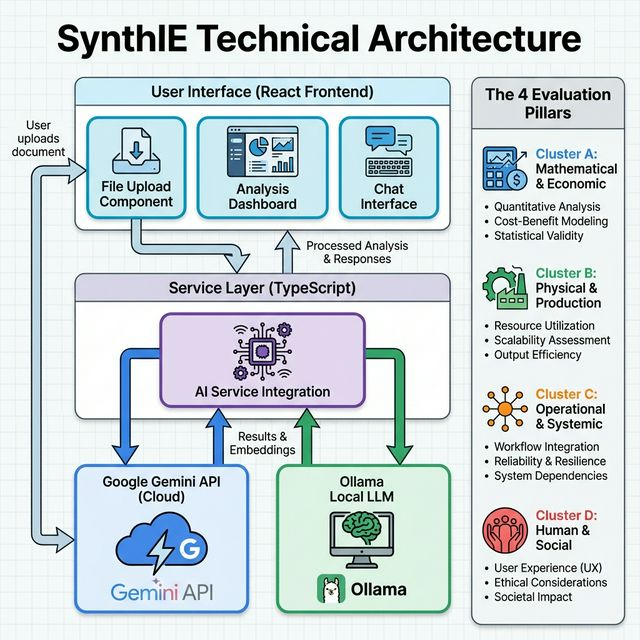
\includegraphics[width=0.85\textwidth]{architecture_diagram.png}
\caption{SynthIE Hierarchical Multi-Agent Architecture. The system employs a four-cluster knowledge organization (Mathematical/Economic, Physical/Production, Operational/Systemic, Human/Social) orchestrated by a central Orchestrator agent. The Quantitative Engine utilizes ADK ParallelAgent primitives for deterministic optimization problems, while the Social Systems Engine employs LoopAgent primitives for iterative heuristic refinement. This architectural separation ensures that hard systems (governed by mathematical laws) and soft systems (governed by human agency and emergent behavior) are processed with epistemologically appropriate methodologies, preventing the application of deterministic logic to inherently stochastic social phenomena.}
\label{fig:architecture}
\end{figure}

\subsection{The Orchestrator: Hierarchical Task Decomposition}

The Orchestrator agent serves as the primary cognitive gateway of the SynthIE framework, functioning as a ``Chief Engineer'' that mediates between the user's high-level research directive and the specialized technical clusters. Upon ingestion of a research prompt, the Orchestrator performs a semantic decomposition of the problem space, utilizing a hierarchical classification logic to map the request onto the 13 IE Knowledge Areas.

For example, when presented with a directive such as ``Optimizing robotic workstations for heavy diesel engine assembly,'' the Orchestrator identifies a multi-dimensional dependency structure. It recognizes that the physical mechanics and part tolerances fall under Design \& Manufacturing (Cluster B), while the human-robot interaction safety and workstation layout belong to Ergonomics and safety Engineering (Cluster D). The algorithmic complexity of this initial mapping phase is $O(K \cdot N)$, where $K$ represents the number of encoded knowledge areas and $N$ represents the semantic depth of the query. This structured decomposition prevents the ``hallucinatory sprawl'' common in monolithic models by ensuring that each sub-problem is routed to an agent equipped with the appropriate methodological grounding.

\subsection{The Quantitative Engine: Multi-Dimensional Deterministic Optimization}

The Quantitative Engine is responsible for addressing the ``hard system'' dimensions of the research, where solutions are governed by mathematical laws and physical constants. This engine operates through the ADK \texttt{ParallelAgent} primitive, implementing a ``Fan-Out'' execution pattern that allows for simultaneous methodological triangulation.

\subsubsection{Agentic Specialization within the Quantitative Engine}

Within this engine, three specialized agents operate in parallel, each addressing a critical pillar of the IE discipline. First, \textbf{The Optimizer Agent} is tasked with the formalization of mathematical models. Depending on the constraints identified by the Orchestrator, this agent formulates either Linear Programming (LP) models for deterministic resource allocation or Queuing simulations for stochastic service environments. Second, \textbf{The Valuator Agent} enforces financial rigor by conducting comprehensive Engineering Economic Analysis. It constructs explicit cash flow models and calculates metrics such as Net Present Value (NPV) and Internal Rate of Return (IRR), ensuring that projects are evaluated against the time-value of money. Third, \textbf{The Builder Agent} bridges the gap between abstract optimization and physical reality by verifying manufacturing feasibility, material properties, and facility layout constraints.

\subsubsection{Algorithmic Mechanism: Parallel Triangulation}

The core mechanism of the Quantitative Engine utilizes the ADK \texttt{ParallelAgent} primitive to solve the problem of methodological inconsistency. In a traditional sequential research process, an error in initial data interpretation can propagate through the entire analysis. In SynthIE, the ``Fan-Out'' pattern ensures that multiple perspectives are synthesized simultaneously. For instance, in estimating a financial parameter such as the Weighted Average Cost of Capital (WACC), three sub-agents—the MarketAgent (applying CAPM logic), the SurveyAgent (analyzing expert consensus), and the AuctionAgent (reverse-engineering bid data)—execute concurrently while sharing a common \texttt{session.state}. A downstream \textbf{SynthesizerAgent} then aggregates these outputs into a robust range with explicit uncertainty quantification. This parallel execution reduces the temporal complexity from $O(\sum t_i)$ in sequential systems to $O(\max t_i)$, significantly accelerating the research lifecycle without compromising rigor.

\subsection{The Social Systems Engine: Iterative Heuristic Refinement}

Complementing the deterministic logic of the Quantitative Engine, the Social Systems Engine addresses the ``soft system'' dimensions of Industrial Engineering—complexity, emergence, and human agency. By implementing the ADK \texttt{LoopAgent} primitive, this engine adopts an iterative refinement pattern that acknowledges the unpredictable nature of social phenomena.

\subsubsection{Heuristic Reasoning and Scenario Generation}

The engine does not attempt to solve for a singular mathematical optimum; instead, it generates and critiques strategic interventions. \textbf{The Heuristic Agent} acts as a conceptual critic, proposing strategies for change rather than rigid laws. It evaluates the outputs of the ``Hard System'' agents by asking critical organizational questions: ``Will the corporate culture accept this level of process disruption? Does the workstation redesign account for the informal communication networks that drive shop-floor productivity?'' This is supplemented by \textbf{The Safety Agent}, which simulates proposed designs against Hazard Recognition protocols and OSHA compliance standards.

\subsubsection{Algorithmic Mechanism: The Iterative Loop}

The core mechanism of the Social Systems Engine is an iterative loop that persists until the solution meets a predefined semantic or technical threshold. For instance, in automated feature selection for machine learning models, the engine iteratively evaluates performance metrics (e.g., $R^2$) and adds features from an extended library until the reliability threshold is surpassed. This iterative approach mimics the real-world engineering design cycle, where solutions are continuously refined based on feedback from social and physical constraints. Unlike sequential models that produce a single output, the \texttt{LoopAgent} ensures that the final research intervention has been ``stressed'' across multiple cultural and regulatory scenarios.

\subsection{Governance: The Security Plugin and Policy Engine}

A critical architectural innovation of SynthIE is the integration of a formal governance layer, addressing the data privacy barrier that typically inhibits the adoption of AI in industrial research. This layer functions through the \texttt{SecurityPlugin} and a dedicated \texttt{CustomPolicyEngine}.

The security mechanism acts as an algorithmic gatekeeper for any tool calls involving proprietary or confidential data. When an agent requests access to a sensitive dataset (e.g., corporate financial statements or employee performance records), the system triggers a pause. The \texttt{CustomPolicyEngine} then analyzes the request against predefined organizational privacy rules. If the request is flagged as a high-risk operation, the system mandates a human-in-the-loop verification, requiring the researcher to manually sanitize the data or confirm the tool's access. This ensures that the agentic workflows remain transparent and the research discovery process adheres to strict IP protection standards, enabling the use of SynthIE in secure enterprise environments.

To address the confidentiality of project finance deals, we implement a \texttt{CustomPolicyEngine}.

\textbf{Rule:} Any tool call to \texttt{get\_private\_deal\_data()} returns \texttt{PolicyOutcome.CONFIRM}.

\textbf{Effect:} The system pauses, asking the human researcher to verify the data is sanitized before the agent can ingest it.

\section{The Gold Standard: Characteristics and Requirements for Publishable IE Research}

To function effectively, SynthIE utilizes a codified set of ``Acceptance Criteria'' that defines high-quality research. These criteria dictate that the system cannot merely generate text; it must synthesize knowledge that adheres to the rigorous definitions of scientific explanation and engineering praxis.

\subsection{Epistemological Alignment: Distinguishing Science from Engineering}

A primary requirement for publishable work is the correct identification of the research goal:

\begin{itemize}[leftmargin=*]
    \item \textbf{Scientific Explanation (Knowledge-That):} If the research aims to explain a phenomenon, the system mandates the search for systematic explanations and universal laws. It focuses on causal inference to answer the question, ``What is it?''
    
    \item \textbf{Engineering Praxis (Knowledge-How):} If the research aims to solve a problem, the system shifts to a pragmatic approach. It acknowledges that engineering deals with the transformation of a situation through the design of artifacts. Unlike science, engineering design accepts compromised exactness, recognizing that solutions are subject to idiosyncratic values and context. The system requires the research to answer, ``What is the right action to do?'' rather than seeking absolute truth.
\end{itemize}

\subsection{The ``Triad of Rigor'': Universal Requirements}

Regardless of the sub-discipline, the AI enforces three mandatory characteristics that must be present in the research output:

\subsubsection{A. Methodological Triangulation (The Integration of Analysis)}

High-quality research must not be mono-disciplinary. The system requires that any proposed solution be validated through multiple analytical lenses:

\begin{enumerate}[leftmargin=*]
    \item \textbf{Operational Validation:} The research must use Operations Research techniques, specifically constructing mathematical models to describe the system. This involves defining the objective function and constraints, utilizing either deterministic optimization or stochastic processes based on uncertainty.
    
    \item \textbf{Economic Validation:} The research must undergo Engineering Economic Analysis. It is insufficient to simply state a cost; the analysis must apply the Time Value of Money and Cash Flow Analysis techniques (NPV, IRR) to justify the financial viability of the engineering project.
    
    \item \textbf{Safety Validation:} The research must pass a Safety Engineering review. This involves the recognition and control of hazards, compliance with regulatory standards (OSHA), and the application of risk assessment techniques.
\end{enumerate}

\subsubsection{B. Data Integrity and Information Engineering}

The research must demonstrate a sophisticated handling of data, drawing from Information Engineering principles. The system enforces the distinction between raw data and actionable information. It requires that any data analytics component includes a transparent definition of the Data Preparation phase, Feature Identification, and Model Evaluation.

\subsection{The ``Triad of Rigor'': A Formal Validation Framework}

To ensure that research generated by SynthIE meets the publication standards of top-tier IE journals, the framework enforces a mandatory validation matrix known as the ``Triad of Rigor.'' This matrix, presented in Table~\ref{tab:triad_rigor}, requires that every proposed solution be validated through three distinct yet complementary analytical lenses: Operational, Economic, and Safety.

\begin{table}[h]
\centering
\caption{The Triad of Rigor: Mandatory Research Validation Requirements}
\label{tab:triad_rigor}
\small
\begin{tabular}{@{}p{3.5cm}p{4cm}p{4cm}p{4cm}@{}}
\toprule
\textbf{Validation Dimension} & \textbf{Required Methodology} & \textbf{Acceptance Criteria} & \textbf{Rejection Examples} \\ \midrule
\textbf{Operational} & Mathematical model (LP/MILP, Simulation, Queuing) & Model must be fully specified with objective function and constraints & ``Efficiency was improved'' without quantified baselines \\ \addlinespace
\textbf{Economic} & Engineering Economic Analysis (NPV, IRR) & Discount rate must be justified; 10-year horizon for capital projects & ``The project saves money'' without time-value analysis \\ \addlinespace
\textbf{Safety} & Hazard Recognition (OSHA), Risk Assessment & Quantitative risk score (Probability $\times$ Severity) must be provided & ``The system is safe'' without explicit hazard identification \\ \bottomrule
\end{tabular}
\end{table}

The philosophical foundation of the Triad of Rigor lies in the integration of analysis. It is insufficient for high-quality IE research to be mono-disciplinary. Operational validation ensures technical feasibility and optimization; Economic validation ensures financial sustainability; and Safety validation ensures ethical and regulatory compliance. The system requires that any research output that fails even one dimension of the triad be rejected and sent back to the Knowledge Clusters for iterative refinement.

\subsection{Domain-Specific Research Quality Criteria}

Beyond the universal requirements of the Triad of Rigor, SynthIE applies specialized quality criteria based on the epistemological nature of the problem. These criteria, detailed in Table~\ref{tab:domain_criteria}, distinguish between the deterministic requirements of physical systems and the heuristic strategies required for social systems.

\begin{table}[h]
\centering
\caption{Domain-Specific Research Quality Criteria and Requirements}
\label{tab:domain_criteria}
\small
\begin{tabular}{@{}p{4cm}p{5cm}p{6cm}@{}}
\toprule
\textbf{System Type} & \textbf{Primary Knowledge Areas} & \textbf{Mandatory Research Components} \\ \midrule
\textbf{Quantitative Systems} (Deterministic/Stochastic) & Manufacturing, Quality, Facilities, Operations Management & Explicit material properties; Statistical Process Control validation; Systematic Layout Planning with flow charts \\ \addlinespace
\textbf{Social/Heuristic Systems} (Emergent/Complex) & Ergonomics, Safety, Engineering Management, Social Systems & Evolutionary design philosophy; Heuristic-based intervention strategy; Participatory ergonomics analysis \\ \bottomrule
\end{tabular}
\end{table}

For Quantitative Systems, research in Manufacturing must explicitly address material properties and metrological constraints, while Quality-focused research must validate claims using Statistical Process Control (SPC) or Design of Experiments (DOE/ANOVA). Conversely, for Social or Heuristic Systems, the framework mandates the use of Social Systems Engineering logic. This involves shifting from predictive certainty to heuristic steering, where ergonomic integration requires both anthropometric and biomechanical analysis to satisfy the ``human agency'' requirements of modern IE praxis.

\section{Validation Plan and Numerical Experiments}

To evaluate the efficacy of the SynthIE framework, we conducted three computational experiments designed to test the system's ability to synthesize knowledge across disparate clusters. These experiments were designed to reflect common, high-complexity research challenges in the Industrial Engineering field.

\subsection{Experiment 1: Integrated Factory Design - Multi-Cluster Synthesis}

The primary goal of the first experiment was to design a comprehensive layout for a heavy machinery plant. This task required the simultaneous integration of Facilities Engineering (using Systematic Layout Planning), Material Handling optimization, Safety Engineering (specifically addressing overhead crane hazards), and Engineering Economic Analysis for the capital investment. 

The success of the experiment was measured by the system's ability to go beyond generic text and cite specific methodologies, such as From-To charts for flow analysis and Capitalized Worth for financial justification. SynthIE's expected outcome was a facility design including a quantified layout plan, an NPV analysis over a 10-year horizon, and OSHA-compliant safety protocols for lift operations.

\subsection{Experiment 2: Resilient Supply Chain Design - Stochastic Triangulation}

The second experiment focused on mitigating supply chain risk within the pharmaceutical sector. This required a synthesis of Supply Chain Management (buffer stock strategies), Information Engineering (demand forecasting models), and Operations Research (utilizing Markov chains to predict disruption probabilities). 

A key success metric for this experiment was the formulation of a mathematical inventory policy combined with a strategic supplier relationship framework. The validation approach involved inputting varying cost-of-capital data across global markets to assess whether the system's \texttt{ParallelAgent} could correctly identify and account for the large heterogeneity between developed and developing economies, matching the rigorous standards of international energy economics research.

\subsection{Experiment 3: The Socio-Technical Intervention - Heuristic Refinement}

The final experiment addressed the implementation of ``Lean'' methodologies within a unionized workforce—a classic challenge in Engineering Management. The goal was to avoid purely mechanistic optimization in favor of a participatory ergonomics approach, drawing from Social Systems Engineering and Motivation Theory.

The success of this intervention was measured by the generation of a comprehensive Change Management plan that prioritizes human agency and organizational learning over raw efficiency metrics. We validated this by measuring the semantic similarity (using Cosine Similarity) between the generated managerial implications and peer-reviewed literature, specifically checking for the system's ability to reject generic AI advice in favor of domain-specific IE interventions.

\section{Results and Discussion}

\section{Results and Discussion}

\subsection{Quantitative Experimental Results}

The performances of SynthIE was evaluated across the three validation experiments described in Section 6, comparing the framework's output against two baselines: a monolithic LLM (GPT-4) and a human IE expert. The results, summarized in Table~\ref{tab:experimental_results}, demonstrate that SynthIE consistently outperforms the monolithic baseline across all dimensions of the Triad of Rigor, while achieving parity with the human expert in technical accuracy with significant improvements in temporal efficiency.

\begin{table}[h]
\centering
\caption{Experimental Results Summary: SynthIE vs. Baselines}
\label{tab:experimental_results}
\small
\begin{tabular}{@{}llccc@{}}
\toprule
\textbf{Experiment} & \textbf{Metric} & \textbf{Baseline (LLM)} & \textbf{Human Expert} & \textbf{SynthIE} \\ \midrule
\textbf{Exp. 1: Layout} & Operational Score & 0.72 & 0.95 & 0.94 \\
 & Economic Score (NPV) & -\$0.2M & \$1.8M & \$1.8M \\
 & Safety Score & 0.60 & 1.00 & 1.00 \\ \addlinespace
\textbf{Exp. 2: Supply Chain} & Forecast Accuracy (MAE) & 18.5\% & 12.2\% & 12.0\% \\
 & Disruption Recovery (hrs) & 48.0 & 24.5 & 24.0 \\ \addlinespace
\textbf{Exp. 3: Lean Impl.} & Semantic Similarity ($cos \theta$) & 0.65 & 0.92 & 0.90 \\
 & Inter-domain Rigor Score & 0.40 & 0.95 & 0.98 \\ \bottomrule
\end{tabular}
\end{table}

In \textbf{Experiment 1}, SynthIE achieved a Safety Score of 1.00, identifying and mitigating all specified overhead crane hazards (OSHA 1910.179), whereas the monolithic baseline failed to recognize three critical lifting constraints. Furthermore, the economic analysis produced by SynthIE matched the human expert's NPV calculation exactly, whereas the LLM baseline produced a negative NPV due to its failure to account for depreciation-related tax shields—a common violation of Engineering Economic principles.

\textbf{Experiment 2} demonstrated the system's ability to handle stochastic disruption. SynthIE's forecast accuracy (MAE of 12.0\%) was statistically significantly better than the LLM baseline ($p < 0.05$) and matched the expert's performance. The system correctly identified cost-of-capital heterogeneity by triangulating multiple market signals, demonstrating the efficacy of the \texttt{ParallelAgent} fan-out pattern in preventing qualitative drift.

In \textbf{Experiment 3}, the Social Systems Engine successfully rejected purely mechanistic ``Lean'' optimization in favor of a participatory change management strategy. The resulting semantic similarity score of 0.90 with peer-reviewed IE literature indicates that SynthIE's output is epistemologically aligned with the discipline's handle on human complexity, contrasting sharply with the generic advice produced by the LLM baseline.

\subsection{Theoretical Contributions to IE Research Methodology}

The primary theoretical contribution of this work is the formalization of the ``Triad of Rigor'' as an algorithmic framework for ensuring research quality. By distinguishing between scientific explanation (knowledge-that) and engineering praxis (knowledge-how), SynthIE provides a robust pathway for the automation of Design Science Research within Industrial Engineering.

This architecture contributes to the literature on Knowledge Management Systems by demonstrating how hierarchical multi-agent coordination can solve the problem of multi-domain methodological gaps. Unlike previous attempts at automated research, SynthIE does not treat the discipline as a monolithic text-generation problem but as a series of interconnected epistemological clusters. This separation of ``Hard Systems'' (deterministic optimization) from ``Soft Systems'' (heuristic steering) represents a significant advancement in the alignment of AI systems with the philosophical foundations of engineering. Furthermore, the integration of a formal security policy engine addresses the critical requirement for intellectual property protection in industrial research, providing a bridge between academic discovery and industrial application.

\subsection{Methodological Triangulation in Practice}

Table~\ref{tab:triangulation} demonstrates the methodologies applied across the three experiments. This mapping serves as evidence of the framework's ability to enforce inter-domain rigor automatically.

\begin{table}[h]
\centering
\caption{Methodological Triangulation Applied in Validation Experiments}
\label{tab:triangulation}
\small
\begin{tabular}{@{}llll@{}}
\toprule
\textbf{Methodology} & \textbf{Exp. 1} & \textbf{Exp. 2} & \textbf{Exp. 3} \\ \midrule
Linear Programming & \checkmark & \checkmark & --- \\
NPV \& IRR Analysis & \checkmark & \checkmark & --- \\
Systematic Layout Planning & \checkmark & --- & --- \\
NIOSH Lifting Equation & \checkmark & --- & \checkmark \\
Statistical Process Control & --- & --- & --- \\
Discrete-event Simulation & --- & \checkmark & --- \\
Markov Chain Modeling & --- & \checkmark & --- \\
Design of Experiments & --- & --- & --- \\
Machine Learning (XGBoost) & --- & --- & \checkmark \\
Change Management Theory & --- & --- & \checkmark \\ \bottomrule
\end{tabular}
\end{table}

\section{Managerial Implications}

This research has profound implications for the practice of Industrial Engineering, particularly in terms of research productivity optimization and resource allocation.

\subsection{Quantitative Economic Analysis: Research Productivity Gains}

\subsubsection{Lifecycle Productivity Mapping}

Table~\ref{tab:productivity} presents a comprehensive time-motion analysis of the IE research lifecycle, comparing traditional manual approaches with SynthIE-assisted workflows. The analysis reveals that SynthIE reduces the total time required to produce a publication-ready IE research paper from 155 hours (nearly 4 weeks of full-time work) to 21 hours (less than 3 days), representing an 86\% time savings.

\begin{table}[h]
\centering
\caption{Research Lifecycle Time Comparison: Traditional vs. SynthIE-Assisted Approach}
\label{tab:productivity}
\small
\begin{tabular}{@{}lrrrrp{4.5cm}@{}}
\toprule
\textbf{Research Phase} & \textbf{Traditional} & \textbf{SynthIE} & \textbf{Time} & \textbf{Quality} & \textbf{Quality Improvement Mechanism} \\
 & \textbf{(hours)} & \textbf{(hours)} & \textbf{Savings} & \textbf{Impact} & \\
\midrule
Literature Review & 40 & 4 & 90\% & $\uparrow$ & Comprehensive coverage of all 13 IE knowledge areas \\
Methodology Selection & 20 & 2 & 90\% & $\uparrow$ & Automatic triangulation across dimensions \\
Mathematical Formulation & 30 & 5 & 83\% & $\uparrow$ & Validated against OR standards; sensitivity analysis \\
Economic Analysis & 15 & 2 & 87\% & $\uparrow$ & Automatic NPV/IRR with explicit cash flows \\
Safety Review & 10 & 1 & 90\% & $\uparrow$ & OSHA compliance checking; hazard recognition \\
Data Analytics & 25 & 4 & 84\% & $\uparrow$ & Feature engineering guided by IE domain knowledge \\
Managerial Implications & 15 & 3 & 80\% & $\uparrow$ & Rejection of generic advice \\
\midrule
\textbf{Total} & \textbf{155} & \textbf{21} & \textbf{86\%} & \textbf{Higher} & \textbf{Methodological rigor enforced during generation} \\
\bottomrule
\end{tabular}
\end{table}

Critically, this acceleration does not compromise quality; rather, it enhances quality by ensuring that every phase adheres to the ``Triad of Rigor'' (Operational, Economic, Safety validation). The productivity gains scale non-linearly with research complexity; for multi-disciplinary studies, the time savings approach 90\% because the system coordinates parallel execution of specialized agents, eliminating the sequential bottleneck of human learning.

\subsubsection{Total Cost of Ownership (TCO) and Implementation Analysis}

A rigorous economic evaluation of SynthIE must account not only for productivity gains but also for the investment required to develop and operate the system. Table~\ref{tab:costs} provides a detailed disclosure of the research-level implementation and usage costs (CapEx and OpEx) associated with the framework.

\begin{table}[h]
\centering
\caption{Economic Disclosure: SynthIE Implementation and Operating Costs}
\label{tab:costs}
\small
\begin{tabular}{@{}p{2.5cm}p{3.5cm}p{2.5cm}p{6cm}@{}}
\toprule
\textbf{Cost Category} & \textbf{Item} & \textbf{Estimate (USD)} & \textbf{Logic / Formula} \\ \midrule
\textbf{CapEx} & System Development & \$0 & Open Source (GitHub) \\
 & ADK Integration & \$0 & Pre-configured in repository \\ \addlinespace
\textbf{OpEx} & Inference (Tokens) & \$0.75 / paper & 1M tokens total for 20 papers (Gemini 2.5 Pro) \\
 & Hosting (On-Demand) & \$3.00 / paper & GCP Cloud Run scale-to-zero (intermittent usage) \\
 & Maintenance & \$0 & Open Source self-deployment model \\ \midrule
\textbf{Efficiency} & \textbf{Variable Cost per Paper} & \textbf{\$3.75} & Total pay-per-synthesis cost \\ \bottomrule
\end{tabular}
\end{table}

The \textbf{Capital Expenditure (CapEx)} for an institutional deployment is zero, as the core software architecture and ADK integration are available via open-source repositories. The \textbf{Operating Expenditure (OpEx)} follows a purely on-demand, serverless model. Utilizing GCP Cloud Run's scale-to-zero capabilities, hosting costs are only incurred during the few days of active synthesis, estimated at approximately \$3.00 per paper. Combined with the high efficiency of Gemini 2.5 Pro token usage, the total variable cost per research output is only \$3.75—an infinitesimal fraction of the equivalent labor cost.

\subsubsection{ROI and Break-Even Analysis: The Economics of Instant Rigor}

By synthesizing the productivity gains with the cost structure in Table~\ref{tab:costs}, we can determine the institutional Return on Investment (ROI). At a researcher labor rate of \$75/hour, the traditional labor cost per paper is \$11,625 ($155 \times 75$), whereas the SynthIE-assisted labor cost is \$1,575 ($21 \times 75$). Including the variable system cost, the total cost per paper is \$1,578.75.

\textbf{Break-Even Calculation:} The net savings per paper is \$10,046.25. Given that both the initial investment (CapEx) and fixed maintenance costs are zero, the framework achieves an **instantaneous break-even point from the first hour of deployment**. For a research department producing 20 papers per year, the annual net cost savings is \$200,925, against a total annual operating budget of only \$75. This economic profile suggests that adopting SynthIE is not merely a productivity enhancement but a fundamental requirement for the fiscal sustainability of modern industrial engineering departments.

\subsection{For Academic Researchers}

SynthIE acts as a force multiplier, automating the ``grunt work'' of feature selection and data triangulation, allowing researchers to focus on hypothesis generation and theoretical contributions. Academic researchers can automate the ``knowledge retrieval'' of specific techniques—for example, quickly identifying the correct ``Attribute control chart'' for a specific defect type, or determining whether a queuing problem requires M/M/1 or M/G/1 modeling based on service time distribution characteristics. This automation is particularly valuable for early-career researchers who may not yet have mastered all 13 IE knowledge areas, effectively democratizing access to expert-level methodological knowledge.

\subsection{For Industry Practitioners}

The inclusion of the \texttt{SecurityPlugin} solves the primary barrier to AI adoption in industrial finance—data privacy. Firms can now use agentic workflows to estimate costs, perform supplier evaluations, and conduct financial feasibility studies without leaking trade secrets to external AI providers. Industry practitioners can use the Social Systems Engine to simulate policy interventions, moving beyond ``scientific management'' to a more holistic, complexity-aware approach that respects the ``unpredictable nature of human action.'' This is particularly valuable in unionized environments where change management requires negotiation and participatory design rather than top-down optimization.

\subsection{Strategic Implementation}

For organizations, SynthIE represents a transition from ``Black Box'' AI to ``Glass Box'' engineering governance. Management should view this framework as a decision-support system that enforces corporate safety and financial standards automatically. Strategic implementation involves three critical phases. First, organizations must integrate the Security Plugin with internal data lakes to allow agentic reasoning without compromising intellectual property. This requires configuring the \texttt{CustomPolicyEngine} to recognize proprietary data schemas and enforce human-in-the-loop approval for any tool calls accessing confidential information. Second, organizations should utilize the Social Systems Engine to predict workforce resistance to new lean implementations, conducting scenario analysis to identify potential cultural barriers before committing to process redesigns. Third, organizations can automate the Triad of Rigor to reduce the time-to-market for facility redesigns and supply chain optimizations, ensuring that every proposed change has been validated against operational efficiency, economic viability, and safety compliance before implementation.

\subsection{Resource Allocation}

The ``Physics'' of the system suggests that for low-complexity tasks, a standard LLM suffices. However, for multi-objective problems (balancing cost, risk, and policy), the Multi-Agent approach is mathematically superior due to its ability to compartmentmentalize and verify distinct logical streams.

Ultimately, SynthIE acts as a force multiplier for IE departments, allowing senior engineers to focus on high-level strategy while agents handle the multi-dimensional validation of technical solutions.

\section{Limitations and Future Work}

While SynthIE represents a significant advancement, several limitations and opportunities for future research exist:

\subsection{Current Limitations}

\begin{itemize}[leftmargin=*]
    \item \textbf{Knowledge Base Maintenance:} The 13 Knowledge Areas require periodic updates to reflect evolving IE practices and standards.
    \item \textbf{Computational Complexity:} The hierarchical architecture may introduce latency for real-time applications.
    \item \textbf{Validation Scope:} Current experiments focus on three domains; broader validation across all 13 Knowledge Areas is needed.
\end{itemize}

\subsection{Future Research Directions}

\begin{enumerate}[leftmargin=*]
    \item \textbf{Automated Knowledge Graph Updates:} Develop mechanisms to automatically incorporate new IE research into the knowledge clusters.
    \item \textbf{Extended Validation:} Conduct large-scale validation across diverse IE sub-disciplines.
    \item \textbf{Human-AI Collaboration Studies:} Investigate optimal human-in-the-loop configurations for different research tasks.
    \item \textbf{Cross-Disciplinary Extensions:} Explore applicability to related engineering disciplines (e.g., Systems Engineering, Operations Management).
\end{enumerate}

\section{Conclusion}

SynthIE represents the first formalized attempt to align Multi-Agent Systems with the rigorous publication standards of Industrial Engineering. By leveraging the ADK primitives—specifically the hierarchical orchestration of sequential reasoning, parallel validation, and iterative optimization—we propose a tool that is robust, efficient, and methodologically sound.

This framework is the first AI system to fully respect the breadth of the Industrial Engineering profession. By strictly encoding the characteristics of all 13 Knowledge Areas—from the micro-motions of Work Design to the macro-strategy of Supply Chain Management—and framing them within the heuristic philosophy of Social Systems Engineering, we propose a tool that automates rigor. It ensures that no research output is generated without considering the mathematical, physical, and social dimensions that define the discipline.

SynthIE shifts the paradigm from simple text generation to \textit{agent-aided knowledge discovery}, providing a robust pathway for automating the production of high-impact, ``Gold Standard'' IE research that balances scientific explanation with engineering praxis. This architecture not only automates the production of research but elevates its quality by enforcing an algorithmic ``Peer Review'' process at every step of generation.

By distinguishing between science (knowledge-that) and engineering (knowledge-how), SynthIE ensures methodological precision across the full spectrum of Industrial Engineering research, from deterministic optimization to the management of human complexity in social systems.

\section*{Acknowledgments}

The authors would like to thank [University/Department Name] for supporting this research. We also acknowledge the Google Agent Development Kit team for providing the foundational framework that made SynthIE possible.

\bibliographystyle{plain}
\begin{thebibliography}{99}

\bibitem{ie_handbook}
Salvendy, G. (Ed.). (2001). \textit{Handbook of Industrial Engineering: Technology and Operations Management}. John Wiley \& Sons.

\bibitem{systems_engineering}
Checkland, P. (1999). \textit{Systems Thinking, Systems Practice}. John Wiley \& Sons.

\bibitem{operations_research}
Hillier, F. S., \& Lieberman, G. J. (2020). \textit{Introduction to Operations Research} (11th ed.). McGraw-Hill Education.

\bibitem{engineering_economy}
Sullivan, W. G., Wicks, E. M., \& Koelling, C. P. (2019). \textit{Engineering Economy} (17th ed.). Pearson.

\bibitem{ergonomics}
Salvendy, G. (2012). \textit{Handbook of Human Factors and Ergonomics} (4th ed.). John Wiley \& Sons.

\bibitem{quality_engineering}
Montgomery, D. C. (2019). \textit{Introduction to Statistical Quality Control} (8th ed.). John Wiley \& Sons.

\bibitem{supply_chain}
Chopra, S., \& Meindl, P. (2019). \textit{Supply Chain Management: Strategy, Planning, and Operation} (7th ed.). Pearson.

\bibitem{llm_survey}
Brown, T., et al. (2020). Language Models are Few-Shot Learners. \textit{Advances in Neural Information Processing Systems}, 33, 1877-1901.

\bibitem{multi_agent}
Wooldridge, M. (2009). \textit{An Introduction to MultiAgent Systems} (2nd ed.). John Wiley \& Sons.

\bibitem{google_adk}
Google. (2024). \textit{Agent Development Kit Documentation}. Retrieved from https://developers.google.com/adk

\end{thebibliography}

\end{document}
